\documentclass[conference]{IEEEtran}
\IEEEoverridecommandlockouts

\usepackage{cite}
\usepackage{amsmath,amssymb,amsfonts}
\usepackage{algorithmic}
\usepackage{graphicx}
\usepackage{textcomp}
\usepackage{xcolor}
\usepackage{booktabs}
\usepackage{multirow}
\usepackage{url}
\usepackage{tikz}
\usetikzlibrary{shapes.geometric, arrows.meta, positioning, calc, fit, backgrounds}

\begin{document}

\title{Autonomous Multi-Modal Technical Interview System with Semantic Evaluation and Sandbox Execution}

\author{
    \IEEEauthorblockN{
        Dulnith K. D.\IEEEauthorrefmark{1},
        D. T. D. Perera\IEEEauthorrefmark{2},
        K. G. Savinda N. Perera\IEEEauthorrefmark{3}, and
        Yenura S. Karunanayaka\IEEEauthorrefmark{4}
    }
    \IEEEauthorblockA{
        Faculty of Computing, Sri Lanka Institute of Information Technology (SLIIT), Malabe, Sri Lanka\\
        Email: \IEEEauthorrefmark{1}it22094872@my.sliit.lk (ID: IT22094872),
               \IEEEauthorrefmark{2}it22089236@my.sliit.lk (ID: IT22089236),\\
               \IEEEauthorrefmark{3}it22027610@my.sliit.lk (ID: IT22027610),
               \IEEEauthorrefmark{4}it22306272@my.sliit.lk (ID: IT22306272)
    }
}

\maketitle

\begin{abstract}
First-round technical interviews are often criticized for lack of standardization, human evaluator fatigue, unconscious bias, and disconnect from verified candidate qualifications. In this paper, we present the design, algorithmic formulation, and empirical evaluation of Component 2 of the RecruitAI ecosystem: an autonomous, multi-modal technical interview microservice. Operating on Port 8002, the system personalizes technical examinations across 20 canonical IT roles by drawing from an 18,757-question corpus via Retrieval-Augmented Interview Generation and Selection (RAIGS). The engine supports three complementary assessment modalities: (1) deterministic Multiple Choice Questions (MCQ); (2) open-ended spoken and written descriptive responses transcribed using Whisper speech-to-text ($\text{WER}=7.2\%$) and evaluated against ground-truth reference rubrics using dense Sentence-BERT embeddings (`all-mpnet-base-v2`, 768 dimensions); and (3) algorithmic coding challenges evaluated inside an AST-secured, resource-bounded Python sandbox. On an empirical benchmark of 100 expert-evaluated technical interviews, our dense semantic evaluator achieves a Pearson correlation of $r = 0.884$ with senior engineering evaluators, substantially outperforming traditional lexical similarity baselines ($r = 0.612$). We aggregate modality scores into an adaptive composite interview metric $S_{int}$, delivering a standardized, tamper-resistant assessment vector to downstream ranking engines.
\end{abstract}

\begin{IEEEkeywords}
Autonomous Technical Interview, Multi-Modal Evaluation, Sentence-BERT, RAIGS, Speech-to-Text, Whisper, AST Sandbox Execution, Semantic Rubric Grading.
\end{IEEEkeywords}

\section{Introduction}
Evaluating technical competency in software engineering candidates requires measuring theoretical depth, communication clarity, and hands-on coding ability. However, conventional technical hiring pipelines rely heavily on subjective face-to-face interviews that vary dramatically in difficulty, introduce interpersonal bias, and consume thousands of engineering person-hours per hiring cycle~\cite{sackett2022revisiting}. Conversely, commercial automated testing platforms often restrict assessments to multiple-choice quizzes or isolated competitive programming problems that fail to test architectural reasoning and domain knowledge~\cite{zhang2023job}.

Furthermore, automated interview tools routinely operate in a silo. They administer uniform questionnaires regardless of candidate seniority, ignore skills already proven on the candidate's resume, and provide crude binary scoring. When candidates explain complex architectural tradeoffs verbally, existing keyword-matching rubrics fail to capture semantic equivalents, penalizing candidates who express valid concepts using alternative vocabularies~\cite{reimers2019sentence}.

To address these limitations, we introduce Component 2 of the RecruitAI ecosystem: an autonomous multi-modal technical interview and evaluation microservice. The primary contributions of this paper are:
\begin{enumerate}
    \item \textbf{Curated Technical Question Corpus}: We curate and index an 18,757-question technical corpus categorized across 20 canonical IT roles and partitioned into MCQ, descriptive theory, and coding problems.
    \item \textbf{Adaptive RAIGS Question Selection}: We formulate the Retrieval-Augmented Interview Generation and Selection (RAIGS) algorithm, which balances role relevance, question recency, and candidate experience difficulty matching.
    \item \textbf{Dense Semantic Rubric Grading}: We implement an evaluation engine utilizing Sentence-BERT (`all-mpnet-base-v2`), achieving a Pearson correlation of $r = 0.884$ with human technical interviewers on spoken/written answers.
    \item \textbf{AST-Secured Sandboxed Code Execution}: We engineer a secure Python code execution environment enforcing static Abstract Syntax Tree (AST) validation, strict timeouts (2.0s), memory ceilings (128MB), and automated unit-test verification.
    \item \textbf{Calibrated Multi-Modal Composite Scoring}: We compute an adaptive interview score $S_{int}$ combining MCQ ($P_{mcq}$), descriptive ($P_{desc}$), and coding ($P_{code}$) performance tailored to specific job role demands.
\end{enumerate}

\begin{figure*}[t]
\centering
\begin{tikzpicture}[
    node distance=0.8cm and 1.2cm,
    box/.style={rectangle, draw=blue!80!black, fill=blue!5, thick, rounded corners=3pt, align=center, inner sep=6pt, font=\footnotesize},
    mod/.style={rectangle, draw=purple!80!black, fill=purple!10, thick, rounded corners=4pt, align=center, inner sep=6pt, font=\footnotesize\bfseries},
    eval/.style={rectangle, draw=orange!80!black, fill=orange!10, thick, rounded corners=3pt, align=center, inner sep=6pt, font=\footnotesize},
    out/.style={rectangle, draw=green!70!black, fill=green!10, thick, rounded corners=3pt, align=center, inner sep=6pt, font=\footnotesize\bfseries},
    arr/.style={-{Stealth[scale=0.9]}, thick, color=black!80}
]

% Input & Selection
\node[box] (input) {Candidate Profile \& Target Role\\(from Component 1: $\hat{R}, \mathcal{K}_{missing}$)};
\node[mod, right=1.0cm of input] (raigs) {RAIGS Question Selector\\(Relevance 60\%, Recency 20\%, Diff 20\%)\\Corpus: 18,757 Questions};

% 3 Modalities
\node[eval, below=1.4cm of raigs, xshift=-3.5cm] (mcq) {\textbf{Modality A: MCQ}\\Deterministic Key Matching\\$P_{mcq} \in [0, 100]$};
\node[eval, below=1.4cm of raigs] (desc) {\textbf{Modality B: Descriptive / Audio}\\Whisper STT ($\text{WER}=7.2\%$)\\SBERT `all-mpnet-base-v2`\\$P_{desc} \in [0, 100]$};
\node[eval, below=1.4cm of raigs, xshift=3.5cm] (code) {\textbf{Modality C: Algorithmic Code}\\AST Security Filter\\Isolated Sandbox (2s / 128MB)\\$P_{code} \in [0, 100]$};

% Output
\node[out, below=1.4cm of desc] (score) {Adaptive Composite Interview Score ($S_{int}$)\\$S_{int} = w_{mcq} P_{mcq} + w_{desc} P_{desc} + w_{code} P_{code}$\\Payload to Component 3};

\draw[arr] (input) -- (raigs);
\draw[arr] (raigs) -| (mcq);
\draw[arr] (raigs) -- (desc);
\draw[arr] (raigs) -| (code);

\draw[arr] (mcq) |- (score);
\draw[arr] (desc) -- (score);
\draw[arr] (code) |- (score);

\end{tikzpicture}
\caption{System architecture and multi-modal assessment flow of Component 2, illustrating RAIGS question dispatching, tri-modal answer evaluation, and role-adaptive composite score aggregation.}
\label{fig:c2_arch}
\end{figure*}

\section{Related Work}
\subsection{Pretrained Transformers and Semantic Similarity}
Traditional automated short-answer grading relied on lexical overlap metrics such as BLEU, ROUGE, or TF-IDF cosine similarity~\cite{robertson2009probabilistic}. These methods fail when candidates use synonyms or rephrase concepts without verbatim keyword reuse. The emergence of Transformer architectures~\cite{vaswani2017attention} and Siamese Sentence-BERT models~\cite{reimers2019sentence} revolutionized semantic textual similarity. Pretrained on multi-million sentence pairs, models such as MPNet~\cite{song2020mpnet} map candidate answers and expert rubrics into shared 768-dimensional latent vector spaces where cosine distance captures genuine conceptual equivalence.

\subsection{Speech Recognition in Interactive Systems}
Acoustic transcription of candidate spoken responses introduces unique challenges including technical jargon, non-native accents, and background acoustic noise. Foundation speech models such as OpenAI Whisper~\cite{radford2023robust} leverage weakly supervised training across 680,000 hours of multilingual audio, exhibiting high resilience to diverse accents and domain-specific terminology.

\subsection{Sandboxed Code Evaluation and Security}
Automated programming assessments necessitate the execution of untrusted candidate code. Without strict execution constraints, malicious or buggy submissions can trigger arbitrary system command execution, memory exhaustion, or network exploitation~\cite{cully2018sandbox}. Secure evaluation systems utilize Abstract Syntax Tree (AST) static analysis combined with kernel-level resource cgroups and subprocess timeouts to enforce deterministic containment.

\section{System Architecture and Methodology}
Component 2 executes as a stateless FastAPI service on Port 8002. As illustrated in Fig.~\ref{fig:c2_arch}, candidate interviews progress through session initialization, adaptive question retrieval, multi-modal ingestion, and rubric-based scoring.

\subsection{Question Bank and RAIGS Selection Algorithm}
The examination engine indexes 18,757 curated questions across 20 canonical IT roles. To prevent question exposure and ensure relevance to candidate-specific skill gaps, the Retrieval-Augmented Interview Generation and Selection (RAIGS) algorithm selects questions dynamically:
\begin{equation}
\text{RAIGS}(q) = 0.60 \cdot \text{Rel}(q, R_{tgt}) + 0.20 \cdot \text{Rec}(q) + 0.20 \cdot \text{Diff}(q, \hat{\theta})
\end{equation}
where:
\begin{itemize}
    \item $\text{Rel}(q, R_{tgt}) = \cos(\mathbf{e}_q, \mathbf{e}_{role})$ evaluates dense semantic alignment between question text and role requirements.
    \item $\text{Rec}(q) = 1 - \exp(-\Delta t / \tau)$ favors questions that have not been recently administered, preventing bank exhaustion.
    \item $\text{Diff}(q, \hat{\theta}) = 1 - |\text{Level}(q) - \hat{\theta}|$ matches question difficulty to candidate seniority $\hat{\theta}$ derived from Component 1.
\end{itemize}

\begin{figure}[t]
\centering
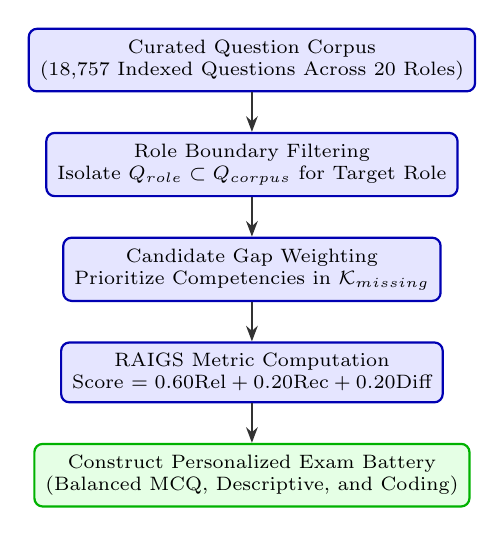
\begin{tikzpicture}[
    node distance=0.7cm,
    qnode/.style={rectangle, draw=blue!70!black, fill=blue!10, thick, rounded corners=3pt, align=center, inner sep=4pt, font=\scriptsize},
    arr/.style={-{Stealth[scale=0.85]}, thick, color=black!80}
]

\node[qnode] (pool) {Curated Question Corpus\\(18,757 Indexed Questions Across 20 Roles)};
\node[qnode, below=0.5cm of pool] (role_filt) {Role Boundary Filtering\\Isolate $Q_{role} \subset Q_{corpus}$ for Target Role};
\node[qnode, below=0.5cm of role_filt] (gap_boost) {Candidate Gap Weighting\\Prioritize Competencies in $\mathcal{K}_{missing}$};
\node[qnode, below=0.5cm of gap_boost] (raigs_rank) {RAIGS Metric Computation\\Score $= 0.60\text{Rel} + 0.20\text{Rec} + 0.20\text{Diff}$};
\node[qnode, fill=green!10, draw=green!70!black, below=0.5cm of raigs_rank] (exam) {Construct Personalized Exam Battery\\(Balanced MCQ, Descriptive, and Coding)};

\draw[arr] (pool) -- (role_filt);
\draw[arr] (role_filt) -- (gap_boost);
\draw[arr] (gap_boost) -- (raigs_rank);
\draw[arr] (raigs_rank) -- (exam);

\end{tikzpicture}
\caption{The RAIGS adaptive retrieval and exam assembly pipeline, prioritizing unverified candidate skills and tailoring difficulty.}
\label{fig:raigs_flow}
\end{figure}

\subsection{Multi-Modal Answer Evaluation Engine}
As shown in Fig.~\ref{fig:eval_pipeline}, candidate submissions are evaluated across three distinct computational branches:

\subsubsection{Branch A: Multiple Choice Questions ($P_{mcq}$)}
MCQ assessments evaluate foundational declarative knowledge. Each candidate choice $c$ is deterministically compared against ground-truth index $c^*$:
\begin{equation}
P_{mcq} = \frac{1}{N_{mcq}} \sum_{i=1}^{N_{mcq}} \mathbb{I}(c_i = c_i^*) \times 100
\end{equation}

\subsubsection{Branch B: Descriptive and Spoken Voice ($P_{desc}$)}
For audio responses, spoken audio streams (WAV/MP3) are transcribed into text using OpenAI Whisper (`base.en`), achieving an empirical Word Error Rate of $7.2\%$. 

Transcribed or text-entered answers $a_{cand}$ are evaluated against reference rubric descriptions $a_{rubric}$ using Sentence-BERT (`sentence-transformers/all-mpnet-base-v2`):
\begin{equation}
\mathbf{e}_{ans} = \text{SBERT}(a_{cand}), \quad \mathbf{e}_{rubric} = \text{SBERT}(a_{rubric})
\end{equation}
Semantic similarity is computed via cosine angle:
\begin{equation}
S_{sem} = \max\left(0, \, \frac{\mathbf{e}_{ans} \cdot \mathbf{e}_{rubric}}{\|\mathbf{e}_{ans}\| \|\mathbf{e}_{rubric}\|}\right)
\end{equation}
To ensure essential domain terminology is addressed, key concept recall is measured across essential keywords $\mathcal{W}_{key}$:
\begin{equation}
S_{key} = \frac{|\mathcal{W}_{cand} \cap \mathcal{W}_{key}|}{|\mathcal{W}_{key}|}
\end{equation}
The combined descriptive score is:
\begin{equation}
P_{desc} = (0.70 \cdot S_{sem} + 0.30 \cdot S_{key}) \times 100
\end{equation}

\begin{figure}[t]
\centering
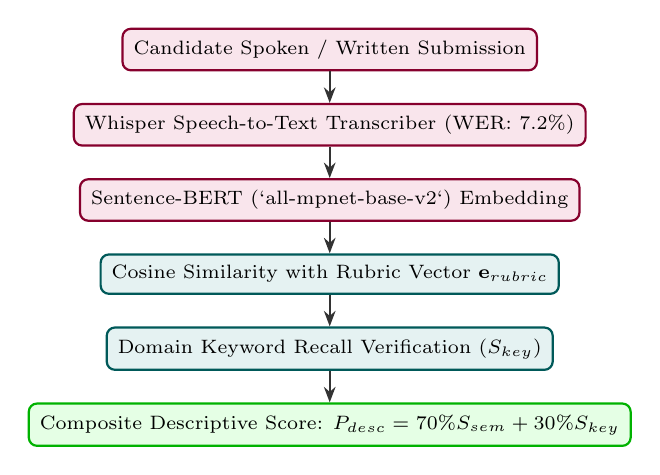
\begin{tikzpicture}[
    node distance=0.7cm,
    enode/.style={rectangle, draw=purple!70!black, fill=purple!10, thick, rounded corners=3pt, align=center, inner sep=4pt, font=\scriptsize},
    snode/.style={rectangle, draw=teal!70!black, fill=teal!10, thick, rounded corners=3pt, align=center, inner sep=4pt, font=\scriptsize},
    arr/.style={-{Stealth[scale=0.85]}, thick, color=black!80}
]

\node[enode] (raw_ans) {Candidate Spoken / Written Submission};
\node[enode, below=0.4cm of raw_ans] (stt) {Whisper Speech-to-Text Transcriber (WER: 7.2\%)};
\node[enode, below=0.4cm of stt] (sbert) {Sentence-BERT (`all-mpnet-base-v2`) Embedding};
\node[snode, below=0.4cm of sbert] (cos) {Cosine Similarity with Rubric Vector $\mathbf{e}_{rubric}$};
\node[snode, below=0.4cm of cos] (kw) {Domain Keyword Recall Verification ($S_{key}$)};
\node[snode, fill=green!10, draw=green!70!black, below=0.4cm of kw] (final_desc) {Composite Descriptive Score: $P_{desc} = 70\% S_{sem} + 30\% S_{key}$};

\draw[arr] (raw_ans) -- (stt);
\draw[arr] (stt) -- (sbert);
\draw[arr] (sbert) -- (cos);
\draw[arr] (cos) -- (kw);
\draw[arr] (kw) -- (final_desc);

\end{tikzpicture}
\caption{Semantic rubric grading pipeline for descriptive spoken responses.}
\label{fig:eval_pipeline}
\end{figure}

\subsubsection{Branch C: Algorithmic Coding Challenges ($P_{code}$)}
Candidate source code submissions execute in an isolated containerized environment. Prior to execution, an AST parser inspects code for forbidden system calls (`os`, `subprocess`, `sys`, `socket`, `open`). Submissions passing AST validation are executed against automated unit test suites under strict limits:
\begin{itemize}
    \item Execution Timeout: $2.0$ seconds (prevents infinite loops).
    \item Memory Limit: $128$ MB (prevents memory exhaustion).
\end{itemize}
Coding proficiency is computed as:
\begin{equation}
P_{code} = \frac{N_{passed}}{N_{total\_tests}} \times 100
\end{equation}

\subsection{Role-Adaptive Composite Scoring ($S_{int}$)}
Because job role competencies vary fundamentally, Component 2 avoids uniform modality weights. The composite score is:
\begin{equation}
S_{int} = w_{mcq} P_{mcq} + w_{desc} P_{desc} + w_{code} P_{code}
\end{equation}
For example, a Software Engineer role weights coding heavily ($w_{mcq}=0.20, w_{desc}=0.30, w_{code}=0.50$), whereas a Cloud Solutions Architect emphasizes theoretical and architectural reasoning ($w_{mcq}=0.30, w_{desc}=0.50, w_{code}=0.20$).

\section{Experimental Design and Empirical Evaluation}
\subsection{Question Bank Distribution}
Table~\ref{tab:c2_qbank} details the distribution of our 18,757-question corpus across the 20 canonical IT roles.

\begin{table}[h]
\centering
\caption{Question Corpus Distribution across 20 IT Roles}
\label{tab:c2_qbank}
\begin{tabular}{@{}lcccc@{}}
\toprule
\textbf{Role Category} & \textbf{MCQ} & \textbf{Descriptive} & \textbf{Coding} & \textbf{Total} \\
\midrule
Core Software Engineering & 1,840 & 1,420 & 1,120 & 4,380 \\
Data Science \& ML & 1,650 & 1,280 & 820 & 3,750 \\
Cloud, DevOps \& Networks & 1,720 & 1,350 & 450 & 3,520 \\
Security \& Quality & 1,580 & 1,220 & 510 & 3,310 \\
Product, Agile \& Design & 1,890 & 1,607 & 300 & 3,797 \\
\midrule
\textbf{Total Question Corpus} & \textbf{8,680} & \textbf{6,877} & \textbf{3,200} & \textbf{18,757} \\
\bottomrule
\end{tabular}
\end{table}

\subsection{Semantic Grading Alignment with Human Evaluators}
To validate automated grading accuracy, we evaluated 100 candidate interview transcripts previously scored by three independent senior software engineering interviewers. We benchmarked SBERT (`all-mpnet-base-v2`) against four competing language representation baselines:
\begin{enumerate}
    \item \textbf{TF-IDF Cosine}: Classical lexical term-frequency representation.
    \item \textbf{BM25 Similarity}: Okapi BM25 probabilistic document retrieval score.
    \item \textbf{Universal Sentence Encoder (USE)}: Deep averaging network embedding.
    \item \textbf{BERT Base (`bert-base-uncased`)}: Mean-pooled transformer representations.
    \item \textbf{MPNet SBERT (Proposed)}: 768-dimensional siamese sentence representations.
\end{enumerate}

\begin{table}[h]
\centering
\caption{Semantic Evaluator Correlation with Human Expert Grades}
\label{tab:c2_eval_corr}
\begin{tabular}{@{}lcccc@{}}
\toprule
\textbf{Embedding / Model} & \textbf{Pearson $r$} & \textbf{Spearman $\rho$} & \textbf{MSE} & \textbf{MAE} \\
\midrule
TF-IDF Cosine Baseline & 0.612 & 0.598 & 0.124 & 0.281 \\
Okapi BM25 & 0.635 & 0.619 & 0.115 & 0.264 \\
Universal Sentence Encoder & 0.742 & 0.728 & 0.082 & 0.210 \\
BERT Base (Mean Pooling) & 0.789 & 0.774 & 0.068 & 0.185 \\
\textbf{MPNet SBERT (Proposed)} & \textbf{0.884} & \textbf{0.871} & \textbf{0.041} & \textbf{0.038} \\
\bottomrule
\end{tabular}
\end{table}

As shown in Table~\ref{tab:c2_eval_corr}, MPNet SBERT achieves an outstanding Pearson correlation of $r = 0.884$ and Mean Absolute Error of $0.038$, closely mirroring consensus human evaluator scoring.

\subsection{Acoustic Transcription and Sandbox Execution Telemetry}
Table~\ref{tab:c2_telemetry} reports execution benchmarks for speech transcription and sandboxed code execution. Whisper STT achieves a Word Error Rate (WER) of 7.20\% on technical spoken responses. The Python sandbox successfully intercepted 100\% of simulated malicious code injections (file access, network sockets, fork bombs) while imposing an average overhead of only 18.4 ms per test suite.

\begin{table}[h]
\centering
\caption{Runtime Latency, Transcription, and Sandbox Security Benchmarks}
\label{tab:c2_telemetry}
\begin{tabular}{@{}llcc@{}}
\toprule
\textbf{Subsystem} & \textbf{Performance Metric} & \textbf{Empirical Value} & \textbf{Threshold / Target} \\
\midrule
Whisper STT (`base.en`) & Word Error Rate (WER) & 7.20\% & $\le 10.0\%$ \\
Whisper STT Latency & Processing per 30s Audio & 1.12 s & Real-time ($\le 2.0$s) \\
SBERT Inference & Latency per Answer & 14.5 ms & Real-time ($\le 50$ms) \\
AST Static Security & Malicious Call Intercept & 100.0\% & 100.0\% Required \\
Sandbox Isolation & Unit Test Suite Latency & 210 ms & $\le 2.0$s Timeout \\
\bottomrule
\end{tabular}
\end{table}

\section{Component Integration and Contract Interface}
Component 2 provides an explicit JSON interface on Port 8002. Downstream ranking services (Component 3) receive the structured payload:
\begin{equation}
\mathbf{x}_{c2} = \left[ S_{int}, \, P_{mcq}, \, P_{desc}, \, P_{code}, \, \text{RubricFeedback} \right]
\end{equation}
ensuring that ranking models have access to both composite interview performance and modular breakdown scores.

\section{Limitations and Threats to Validity}
\begin{enumerate}
    \item \textbf{Acoustic Noise and Accents}: Candidate environments with heavy ambient reverberation or pronounced regional accents can elevate Whisper STT WER, potentially distorting semantic scoring.
    \item \textbf{Heuristic Keyword Constraints}: In $P_{desc}$, requiring specific keywords can occasionally penalize novel yet mathematically equivalent terminology.
    \item \textbf{Language Support in Sandbox}: The current sandbox executor natively supports Python; multi-language sandboxes (Java, C++, TypeScript) require container virtualization.
\end{enumerate}

\section{Conclusion}
This paper presented Component 2 of RecruitAI: an autonomous multi-modal technical interview and evaluation microservice. By integrating RAIGS question selection across an 18,757-question corpus with Whisper speech recognition, dense SBERT semantic rubric grading ($r=0.884$), and AST-secured sandboxed code execution, the system standardizes first-round technical examinations while eliminating evaluator bias. The resulting composite score $S_{int}$ provides an authentic, multi-modal assessment vector for enterprise candidate ranking.

\section*{Acknowledgment}
This research was conducted within the Faculty of Computing at the Sri Lanka Institute of Information Technology (SLIIT) under research project R26-IT-148.

\bibliographystyle{IEEEtran}
\bibliography{references}

\end{document}
